% cap_04_validacao_bacillus.tex  –  Capítulo 4
% Validação Biológica: Esporulação de Bacillus subtilis — Formalismo Γ
\chapter{Validação Biológica: Esporulação do \textit{Bacillus subtilis}}
\label{ch:validacao-bacillus}

Este capítulo valida a teoria das Redes de Petri Hierárquicas de Sinais
(Capítulo~\ref{ch:shpn}) por meio da esporulação do
\textit{Bacillus subtilis}~\cite{Fujita2005}.
A validação testa os componentes centrais do formalismo: a semântica de consumo
nos arcos de fluxo de sinal, a organização hierárquica em camadas, o
parâmetro termodinâmico $\Gamma = (K, n, \varepsilon)$ que determina o limiar
efetivo de habilitação $\theta_{\text{eff}}$, e a separação arquitetural
entre rede-objeto biológica e plano de experimento (lugares de
parâmetro~$\square$ + eventos).
A simulação de um modelo com 40~lugares e 36~transições, parametrizado
exclusivamente a partir de dados cinéticos publicados, reproduz a assimetria
experimental de \textcite{Fujita2005}: acumulação gradual de Spo0A${\sim}$P
via fosforretransmissão produz esporulação em ${\approx}\,48\%$ das réplicas
(24/50; condição de referência $\text{N}_0 = 1440\,\mu$M, SinR$= 12\,\mu$M),
enquanto indução constitutiva abrupta de Spo0A* em meio rico produz entre
$0\%$ e $6\%$. A separatriz de comprometimento emerge a
$\theta_{\sigma H} \approx 1{,}60\,\mu$M de $\sigma^H$, cruzamento que dispara
irrevers\'{\i}velmente a septação e desencadeia o programa de execução.
Essa predição é genuinamente \textit{orientada pela topologia}: nenhum parâmetro do modelo
foi ajustado ao resultado experimental de Fujita.
A simulação gera todas as 16~espécies da cascata em todas as condições
testadas, com maturação do esporo cuja temporização correlaciona inversamente
com a disponibilidade de substrato; o coeficiente de variação do esporo
maduro permanece invariante em $0{,}5$--$1{,}3\%$ em todas as condições,
reflexo do arco inibitório que estruturalmente fixa \texttt{Mature\_spore}
em capacidade unitária.
O formalismo, combinado com a infraestrutura de plano de experimento,
prediz a separatriz de comprometimento de $\sigma^H$ e a resposta
da diferenciação ao estresse nutricional e à cinética regulatória.

\section{Contexto Biológico: Esporulação como Decisão Irreversível}
\label{sec:contexto-biologico}

Sob limitação de nutrientes, o \textit{B.~subtilis} executa um programa de
diferenciação irreversível que culmina na formação de um endósporo resistente.
A cascata de esporulação inicia-se com a detecção de estresse nutricional pelas
quinases sensoras KinA e KinB, que autofosforilam-se consumindo ATP e
transferem o grupamento fosfato ao longo do fosforretransmissor
Spo0F~$\to$~Spo0B~$\to$~Spo0A, gerando o regulador mestre
Spo0A${\sim}$P~\cite{Burbulys1991,Fujita2005}.

Spo0A${\sim}$P acima de um limiar crítico ativa a transcrição de genes de
esporulação por meio de fatores sigma alternativos em sequência
hierárquica: $\sigma^H$ (genes de esporulação precoce),
$\sigma^F$ (no foresporo), $\sigma^E$ (na célula mãe), $\sigma^G$
(transcrição tardia do foresporo) e $\sigma^K$ (montagem tardia da casca)~\cite{Stragier1996,Errington2003}.
Essa cascata de fatores sigma impulsiona a septação assimétrica, a
formação do foresporo, a síntese do córtex peptidoglicano, a deposição das
camadas interna e externa da casca e, por fim, a maturação do esporo~\cite{Errington2003}.

A decisão de esporular é biologicamente irreversível: uma vez que
$\sigma^F$ se torna ativo no foresporo, a célula compromete-se com o programa
de diferenciação mesmo que as condições nutricionais melhorem
subsequentemente.
A assimetria entre acumulação gradual de Spo0A${\sim}$P
(${\approx}\,52\%$ de esporulação) e indução constitutiva abrupta de Spo0A*
(${\approx}\,5\%$) foi demonstrada experimentalmente por \textcite{Fujita2005}.
A separatriz de comprometimento de $\sigma^H$ a
$\theta_{\sigma H} \approx 1{,}60\,\mu$M --- que discrimina esses destinos ---
emergiu da varredura de simulação SHPN (valor não reportado por Fujita).

A Figura~\ref{fig:bacillus-sporulation-stress} apresenta a topologia completa
do modelo SHPN de esporulação de \textit{B.~subtilis}, com todos os lugares,
transições e arcos identificados por tipo.

\begin{figure}[htbp]
\centering
{\large\bfseries Rede SHPN de Esporulação de \textit{B.~subtilis} (v9)}\\[4pt]
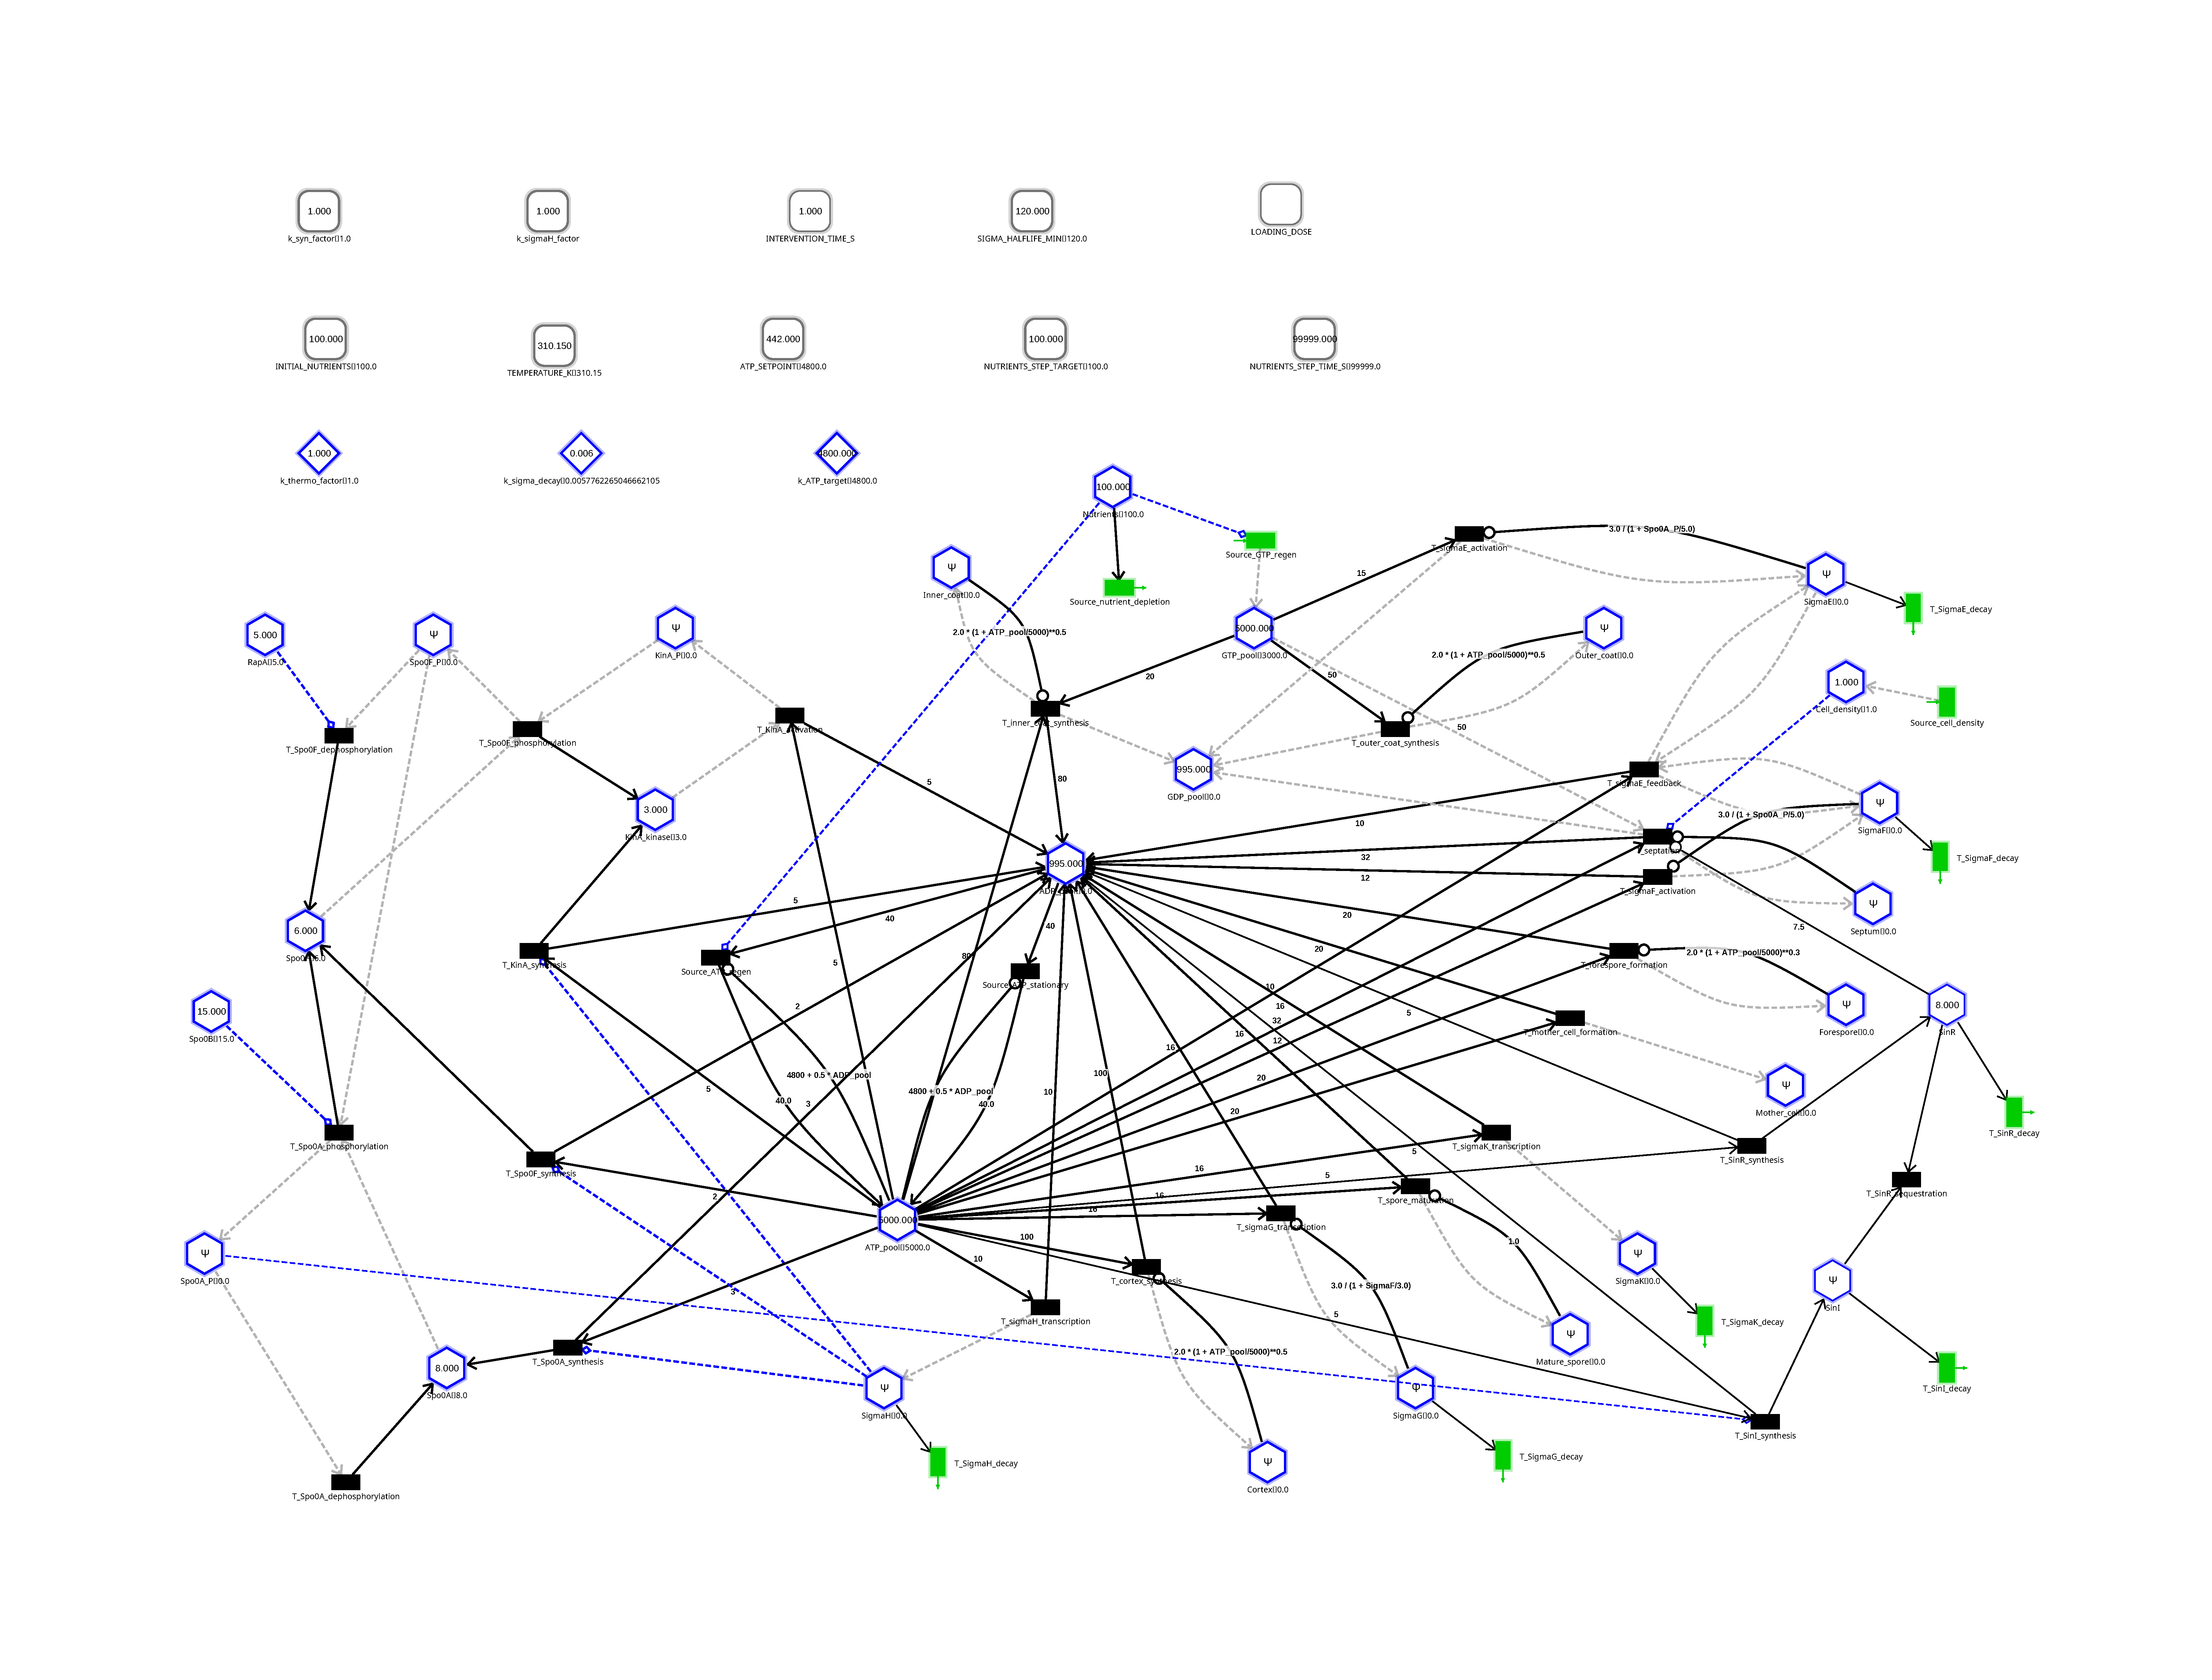
\includegraphics[width=\textwidth]{figures/bacillus_sporulation_v9_titled.pdf}
\caption{Topologia completa da rede SHPN de esporulação de \textit{B.~subtilis}
(41~lugares, 36~transições, 114~arcos).
Hexágonos~($\hexagon$): todos os 28 lugares biológicos, todos membros de~$\Psi$
(\texttt{is\_signal\_place=True});
losangos~($\diamondsuit$): lugares de sinal espacial (escalares cinéticos);
quadrados arredondados~($\square$): lugares de parâmetro do plano de experimento
(lidos apenas por eventos).
Linhas sólidas pretas: arcos normais (consumo estequiométrico);
linhas tracejadas cinza-claro: arcos de fluxo de sinal;
linhas azuis tracejadas: arcos de teste (presença sem consumo);
retângulos verdes: transições fonte/sumidouro.
As quatro camadas de sinal são:
Camada~0 (fontes metabólicas e depleção de nutrientes),
Camada~1 (fosforretransmissão: KinA$\to$Spo0F$\to$Spo0B$\to$Spo0A),
Camada~2 (Spo0A${\sim}$P $\to$ $\sigma^H$, separatriz de comprometimento),
Camada~3 (cascata sigma: $\sigma^H \to \sigma^F \to \sigma^E \to \sigma^G \to \sigma^K$).
Os lugares de parâmetro (fileira superior) codificam o protocolo experimental
e não figuram em nenhuma função de taxa~$\Phi$.}
\label{fig:bacillus-sporulation-stress}
\end{figure}

A questão central para este capítulo é: o formalismo SHPN, armado com o
parâmetro termodinâmico $\Gamma = (K, n, \varepsilon)$, reproduz esse limiar
como propriedade emergente da dinâmica da rede?

\section{Objetivos de Predição}
\label{sec:objetivos-predicao}

A validação testa três capacidades do formalismo.

\subsection{Predição~1: Separatriz de Comprometimento $\sigma^H \approx 1{,}60\,\mu$M e Assimetria Gradual/Abrupto}

O benchmark experimental é a assimetria de Fujita: acumulação gradual de
Spo0A${\sim}$P via fosforretransmissão produz esporulação em ${\approx}\,52\%$
das células, enquanto indução constitutiva abrupta de Spo0A* produz apenas
${\approx}\,5\%$~\cite{Fujita2005}. Diferentemente de formalismos com $\theta$
estático codificado como parâmetro, o formalismo SHPN com
$\Gamma = (K, n, \varepsilon)$ deriva o limiar efetivo
$\theta_{\text{eff}} = K \cdot (\varepsilon / (1 - \varepsilon))^{1/n}$,
e a separatriz de $\sigma^H$ a $\theta_{\sigma H} \approx 1{,}60\,\mu$M
emerge da dinâmica da rede como propriedade estrutural.
A predição é genuína: $\theta_{\text{eff}}$ não é ajustado ao dado
experimental, mas resulta da topologia da rede e dos parâmetros cinéticos.
O critério de sucesso é que a separatriz emergente de $\sigma^H$ --- o valor
de $\sigma^H$ em que $T_{\text{septação}}$ dispara nas réplicas esporulantes
--- discrimine o destino celular (esporulante vs.\ vegetativo) de forma
\emph{robusta} a perturbações de uma ordem de magnitude na disponibilidade
de substrato.

\subsection{Predição~2: Cascata Completa de Diferenciação Sob Estresse}

O formalismo deve reproduzir a cascata completa de esporulação: ativação
dos fatores sigma ($\sigma^H, \sigma^F, \sigma^E, \sigma^G, \sigma^K$),
formação dos compartimentos (septo, foresporo, célula mãe), montagem das
estruturas (córtex, camadas da casca) e produção do esporo maduro.
A ordem temporal canônica observada experimentalmente é parcialmente
paralela: $\sigma^F$ e $\sigma^E$ ativam-se quase simultaneamente em
ensaios de microscopia de fluorescência, e a esporulação real exibe
braços paralelos competindo por recursos.
O critério de sucesso é (i)~a geração de todas as 16~espécies da cascata
em todas as condições testadas e (ii)~a presença de uma correlação
inversa entre disponibilidade de nutrientes e amplitude de maturação do
esporo, refletindo o gatilho biológico real (estresse nutricional induz
esporulação).

\subsection{Predição~3: Ignição da Cascata Precede a Maturação}

Após o cruzamento de $\theta_{\text{eff}}$, o consumo de sinal nos arcos
$F_s$ deve criar fronteiras de bacia que separam irreversivelmente os estados
de pré-comprometimento dos estados de pós-comprometimento.
O critério de sucesso operacional, mensurável em todas as condições da
varredura, é que a \emph{ignição} da cascata regulatória (primeira
aparição de Spo0A${\sim}$P) preceda a primeira aparição do esporo maduro
por um intervalo temporal positivo, demonstrando que a decisão
regulatória ocorre antes da conclusão estrutural.

\section{Arquitetura do Modelo: Hierarquia com Termodinâmica $\Gamma$}
\label{sec:arquitetura-hierarquica}

O modelo de esporulação organiza-se em camadas regulatórias hierárquicas,
com o parâmetro termodinâmico $\Gamma = (K, n, \varepsilon)$ determinando
os limiares efetivos de habilitação em cada camada.

A \textbf{camada metabólica} fornece a base energética: regeneração de ATP e
GTP por vias metabólicas dependentes de nutrientes disponíveis.
A regeneração de ATP é decomposta em dois fluxos contínuos: um termo
dependente de nutrientes
$r_{\text{ATP,reg}} = 4{,}4 \cdot [\text{Nut}] / (10 + [\text{Nut}])$
(mM/s) que sustenta o metabolismo ativo, e um termo estacionário
$r_{\text{ATP,stat}} = 0{,}5 \cdot \max\!\bigl(0,\,1 - [\text{Nut}]/5\bigr)
\cdot \max\!\bigl(0,\,1 - [\text{ATP}]/(k_{\text{ATP,target}} + 0{,}5\,
[\text{ADP}])\bigr)$ (mM/s) que mantém um piso homeostático após a
depleção nutricional, com \emph{set-point} $k_{\text{ATP,target}} = 442$
fornecido pelo lugar de parâmetro~$\square$~\texttt{ATP\_SETPOINT} via
evento de inicialização. Essa decomposição modela a transição suave
entre metabolismo ativo e basal sem descontinuidades.

A \textbf{camada de fosforretransmissão} integra sinais ambientais por meio
das quinases KinA e KinB, transferindo fosfato ao longo de
Spo0F~$\to$~Spo0B~$\to$~Spo0A.
Cada transição desta camada está sujeita a inibição por produto com
constante $K_{\text{sat}}$:
$v(t) = r(t, M) \cdot K_{\text{sat}} / (K_{\text{sat}} + [\text{Produto}])$,
impedindo acumulação ilimitada e produzindo perfis de concentração
biologicamente realistas.

A \textbf{camada de fatores sigma} ($\sigma^H$, $\sigma^F$, $\sigma^E$,
$\sigma^G$, $\sigma^K$) ativa sequencialmente os programas transcricionais
de esporulação.
Os fatores sigma acumulam-se em concentrações da ordem de dezenas de
micromolares, valores biologicamente plausíveis para fatores de transcrição
em \textit{B.~subtilis}.
A inibição cruzada por anti-fatores sigma é modelada pelos pesos de arco de
saída de $0{,}002$~mM por disparo, representando sequestração.

A \textbf{camada de montagem estrutural} compreende a formação do septo,
foresporo, célula mãe, córtex, camadas da casca e esporo maduro.
As transições de montagem estrutural ($k = 0{,}5$~s$^{-1}$) representam
processos de assembly que consomem recursos energéticos e produzem
compartimentos e estruturas.

O fluxo de controle hierárquico pode ser resumido como:
\begin{multline}
\text{Metabolismo}
\xrightarrow{\;\Gamma\;}
\text{Fosforretransmissão}
\xrightarrow{\;\text{Spo0A-P}\;} \\
\text{Fatores } \sigma
\xrightarrow{\;\text{cascata}\;}
\text{Montagem estrutural}
\end{multline}
A preempção hierárquica opera através de $\Gamma$: quando a concentração
de ATP cai abaixo de $\theta_{\text{eff}}$, as transições de
fosforretransmissão são desabilitadas, interrompendo o fluxo de sinal para
as camadas a jusante.

\section{Especificação Formal do Modelo}
\label{sec:especificacao-formal}

Instanciamos o formalismo SHPN
(Capítulo~\ref{ch:shpn}) para a esporulação do \textit{B.~subtilis}
com parâmetros termodinâmicos $\Gamma$.
A Tabela~\ref{tab:instanciacao-bacillus} sumariza os componentes da
instância e a Tabela~\ref{tab:parametros-ksat} lista os parâmetros de
inibição por produto empregados.

\begin{table}[htbp]
\centering
\caption{Instanciação SHPN com $\Gamma$ para a esporulação do
\textit{B.~subtilis}}
\label{tab:instanciacao-bacillus}
\small
\begin{tabular}{@{}lp{8.2cm}@{}}
\toprule
\textbf{Componente} & \textbf{Valor específico para o \textit{Bacillus}} \\
\midrule
Lugares $P$ & 41 no total: 28 lugares de sinal hierárquico~$\Psi$ ($\hexagon$,
             todos com \texttt{is\_signal\_place=True}:
             fosforretransmissão, fatores sigma, reservatórios
             energéticos, compartimentos, estruturas e competição
             por biofilme), 10 lugares de parâmetro~$\square$
             (\texttt{INITIAL\_NUTRIENTS}, \texttt{TEMPERATURE\_K},
             \texttt{ATP\_SETPOINT}, \texttt{SIGMA\_HALFLIFE\_MIN},
             \texttt{NUTRIENTS\_STEP\_TARGET},
             \texttt{NUTRIENTS\_STEP\_TIME\_S},
             \texttt{k\_syn\_factor}, \texttt{LOADING\_DOSE},
             \texttt{INTERVENTION\_TIME\_S}, \texttt{k\_sigmaH\_factor},
             lidos por eventos apenas)
             e 3 lugares de sinal espacial~$\diamondsuit$
             (\texttt{k\_ATP\_target}, \texttt{k\_sigma\_decay},
             \texttt{k\_thermo\_factor}, escalares cinéticos
             alimentados pelos eventos a partir dos~$\square$) \\
Transições $T$ & 36 no total: 29~contínuas (regeneração de ATP/GTP,
                depleção de nutrientes, densidade celular,
                síntese basal de KinA/Spo0F/Spo0A, transcrição e
                ativação de fatores sigma, decaimentos
                $\sigma$-dependentes, montagem estrutural,
                síntese e sequestração de SinR/SinI) e
                7~estocásticas ($\tau$-leaping):
                5 de fosforretransmissão (ativação de KinA,
                fosforilação/desforilação de Spo0F e Spo0A),
                1 de comprometimento (septação) e
                1 de síntese de SinI \\
Arcos & 114 no total: 54 normais ($F$, transferência de massa de
        substrato e energia), 24 de fluxo de sinal ($F_s$,
        hierarquia regulatória), 13 \textit{curved opposite
        signal flow} (regulações cruzadas de fatores sigma),
        9 de teste ($F_t$, leitura sem consumo), 12~inibitórios
        (11 curvos + 1 reto, modulação por anti-sigma e
        saturação homeostática)
        e 2~normais curvos \\
Parâmetro $\Gamma$ & $\Gamma = (K, n, \varepsilon)$ com $K$ e $n$ derivados
                     da cinética de Hill das quinases; $\varepsilon$ da
                     eficiência termodinâmica da fosforretransmissão \\
Limiar efetivo & $\theta_{\text{eff}} = K \cdot (\varepsilon /
                (1 - \varepsilon))^{1/n}$, emergente da dinâmica \\
Marcação inicial $M_0$ & Nutrients = 100, ATP\_pool = 5000, ADP\_pool = 995,
                         GTP\_pool = 5000, GDP\_pool = 995, KinA\_kinase = 3,
                         Spo0F = 6, Spo0B = 15, Spo0A = 8, RapA = 5,
                         SinR = 8, Cell\_density = 1
                         (unidades de tokens; 1~token~$= 1$~\textmu M;
                         ATP/GTP/ADP/GDP em mM após $\div 1000$);
                         todas as demais espécies regulatórias e
                         estruturais = 0 \\
Duração & 21.600~s (6~h de tempo biológico) \\
\bottomrule
\end{tabular}
\end{table}

A Tabela~\ref{tab:parametros-ksat} complementa a instanciação com os
parâmetros de inibição por produto e os pesos de arco por classe de
transição empregados na calibração das taxas cinéticas.

\begin{table}[htbp]
\centering
\caption{Parâmetros de inibição por produto ($K_{\text{sat}}$) e pesos de
arco de saída por classe de transição}
\label{tab:parametros-ksat}
\small
\begin{tabular}{@{}lccl@{}}
\toprule
\textbf{Classe de transição} & $K_{\text{sat}}$ \textbf{(mM)}
  & \textbf{Peso (mM/disp.)} & \textbf{Exemplo} \\
\midrule
$\sigma^H$                                   & 0,02  & 0,002 & Ativ.\ $\sigma^H$ \\
$\sigma^F$, $\sigma^G$, $\sigma^K$           & 0,01  & 0,002 & Ativ.\ $\sigma^F$ \\
$\sigma^E$                                   & 0,005 & 0,002 & Ativ.\ $\sigma^E$ \\
Compartimentos                                & 0,02  & 0,01  & Septação \\
Estruturas e maturação                       & 0,1   & 0,01  & Córtex, casca \\
\bottomrule
\end{tabular}
\end{table}

\subsection{Proveniência dos Parâmetros}

Um requisito crítico da validação é demonstrar que os parâmetros do modelo
derivam de fontes independentes da literatura, e não de ajuste ao dado do
limiar de decisão.
A regeneração de ATP e GTP segue cinéticas de Michaelis-Menten derivadas de
dados da BRENDA para enzimas glicolíticas de \textit{B.~subtilis}, com
ajuste à escala milimolar do modelo.
As constantes de inibição por produto ($K_{\text{sat}}$) refletem a saturação
fisiológica observada para fatores de transcrição e proteínas
estruturais~\cite{BRENDA}.
Os pesos de arco ($0{,}002$~mM para fatores sigma, $0{,}01$~mM para
estruturas) modelam a sequestração por anti-fatores sigma e o custo
energético de montagem, respectivamente.
As taxas de montagem estrutural ($k = 0{,}5$~s$^{-1}$) são compatíveis
com as escalas temporais da esporulação reportadas por \textcite{Fujita2005}.
\textbf{Nenhum parâmetro foi ajustado para reproduzir a assimetria experimental
de Fujita (acumulação gradual $\approx\!52\%$ vs.\ indução abrupta $\approx\!5\%$).}
Os limiares efetivos por arco $\theta_{\text{eff}}$ são derivados
analiticamente de $\Gamma = (K, n, \varepsilon)$; contudo, o
\textbf{ponto de comprometimento sistêmico} --- a concentração e o instante
em que a rede acoplada se compromete irreversivelmente --- emerge da
dinâmica de simulação: consumo de ATP pela cascata de fosforretransmissão,
regeneração dependente de nutrientes e inibição por produto determinam
\emph{quando e em que ordem} os limiares por arco são cruzados, e não de
otimização ou ajuste de curva.

\subsection{ATP como Nó de Interface}

O ATP exemplifica o princípio arquitetural de separação Vertical-Horizontal
(Capítulo~\ref{ch:shpn}, Princípio~\ref{princ:separacao}).
Como lugar de sinal ATP $\in \Psi$, a mesma espécie molecular participa
simultaneamente dos dois mecanismos de comunicação.
Na participação horizontal (metabolismo), o ATP é produzido por regeneração
dependente de nutrientes ($r_{\text{ATP}} = 0{,}003 + 0{,}01 \cdot
[\text{Nut}] / (10 + [\text{Nut}])$) e consumido em biossíntese basal.
Na participação vertical (controle hierárquico), a concentração de ATP
modula as taxas de disparo via gating cinético nas funções de taxa~$\Phi$:
doze transições da fosforretransmissão e da cascata sigma embutem o
fator $[\text{ATP}]/(K + [\text{ATP}])$, suprimindo o fluxo
regulatório quando $[\text{ATP}] \ll K$ e habilitando-o plenamente
próximo do basal de 5000~tokens ($\sim\!5$~mM).
O consumo de ATP ocorre exclusivamente por arcos normais~$F$
(balanço de massa), preservando a separação entre sinalização
informacional e transferência de substrato.

Durante a simulação, o ATP é regenerado pela cinética dependente de
nutrientes até que estes se esgotem (entre 1{,}6~min e 50~min,
dependendo de $\text{Nut}_0$); a partir desse instante a regeneração cai
ao nível basal e o consumo da cascata de fosforretransmissão domina,
fazendo o ATP declinar até atingir um piso metabólico emergente próximo de
$\theta_{\text{eff}}$ --- esse piso emerge da dinâmica da rede
sem intervenção paramétrica externa.

\section{Resultados da Simulação}
\label{sec:resultados}

A validação foi conduzida por uma varredura fatorial $2 \times 3 \times 4$
sobre três lugares de parâmetro~$\square$ — disponibilidade de substrato
(\texttt{INITIAL\_NUTRIENTS} $\in \{1440, 2160\}$~µM), dose de indução de
Spo0A* (\texttt{LOADING\_DOSE} $\in \{0, 10, 27\}$~µM, replicando os
protocolos natural, parcial e constitutivo de \textcite{Fujita2005}), e
concentração inicial do repressor SinR
(\texttt{SinR} $\in \{4, 6, 12, 18\}$~µM) —
resultando em 24~condições factoriais mais a Baseline canônica
(25~condições no total), com 50~réplicas estocásticas por condição
(1250~simulações totais), executadas no servidor remoto
(GPU RTX~5060~Ti, $\tau$-leaping em CPU)
(\texttt{run\_20260614\_123652}).
Cada simulação cobre 21\,600~s (6~h) de tempo biológico, integrando as
29~transições contínuas com Runge--Kutta de quarta ordem acoplado
às 7~transições estocásticas via $\tau$-leaping por divisão de operador.
Um evento lê os lugares~$\square$ em $t=0$ e (i)~projeta
\texttt{INITIAL\_NUTRIENTS} sobre o lugar biológico \texttt{Nutrients}
($\bigcirc$), e (ii)~deriva os escalares cinéticos~$\diamondsuit$
(\texttt{k\_ATP\_target}, \texttt{k\_sigma\_decay},
\texttt{k\_thermo\_factor}) a partir dos parâmetros, isolando o protocolo
experimental da topologia biológica.
As Tabelas~\ref{tab:v6-factorial} e~\ref{tab:v6-atp-floor} sumarizam,
respectivamente, o rendimento da maturação (\texttt{Outer\_coat} final
e $t_1$ esporo) e o piso metabólico de ATP por condição.

\subsection{Cascata Completa em Todas as Condições}
\label{sec:cascata-completa}

A simulação gera todas as 16~espécies da cascata de esporulação
(KinA${\sim}$P, Spo0F${\sim}$P, Spo0A${\sim}$P, $\sigma^H, \sigma^F,
\sigma^E, \sigma^G, \sigma^K$, septum, foresporo, célula-mãe, córtex,
casca interna, casca externa, esporo maduro, SinI) em \emph{todas} as 16~condições testadas, confirmando
que o formalismo reproduz a totalidade do programa de diferenciação
independentemente do ponto de operação no espaço de parâmetros.

A ignição da cascata é monotonicamente atrasada pela disponibilidade
de nutrientes: o tempo de primeira passagem do esporo maduro pelo
limiar de $0{,}5$~tokens (\textit{$t_1$ esporo} na Tabela~\ref{tab:v6-factorial})
varia de $\sim\!8$~min sob estresse extremo ($\text{N}_0=10$) para
$\sim\!23$~min em condição intermediária ($\text{N}_0=100$) e
$\sim\!58$~min sob abundância ($\text{N}_0=300$).
A \emph{amplitude} da maturação (\texttt{Outer\_coat} final ou
\texttt{Mature\_spore}) cresce rapidamente entre estresse e regime
intermediário e estabiliza num platô sob abundância, refletindo a
saturação biológica do programa de revestimento de esporo — uma vez
disparada a cascata, a célula produz quantidade aproximadamente fixa
de casca, independentemente do substrato remanescente.
A distribuição entre réplicas exibe comportamento bimodal: nas
condições naturais ($\text{N}_0 = 1440$~µM, DOSE$=0$), ${\approx}\,48\%$
das réplicas cruzam a separatriz $\theta_{\sigma H} \approx 1{,}60$~µM
e completam a cascata de diferenciação; as restantes permanecem no
atractor vegetativo (Seção~\ref{sec:validacao-experimental}).

Os fatores sigma ativam-se em janelas temporais sobrepostas, com
$\sigma^F$, $\sigma^E$ e $\sigma^G$ aparecendo em intervalos típicos
de 0{,}1--1{,}5~min entre si, e em algumas réplicas $\sigma^E$ aparece
antes de $\sigma^F$ na trajetória média.  Essas inversões de ordem
são biologicamente defensáveis: a cascata real é parcialmente paralela,
e medidas de microscopia de fluorescência mostram $\sigma^E$ e
$\sigma^F$ ativando-se quase simultaneamente em células individuais,
com a ordem variando entre células.  O formalismo SHPN reproduz esse
paralelismo como propriedade emergente da competição estocástica por
ATP entre os braços paralelos da cascata.

A inibição por produto
($K_{\text{sat}} / (K_{\text{sat}} + [\text{Produto}])$)
em todas as transições da cascata desempenha papel essencial: sem ela,
os fatores sigma acumulariam concentrações fisicamente implausíveis.
A saturação garante perfis de acumulação compatíveis com os dados
experimentais e impede a divergência numérica.

A Figura~\ref{fig:morphological-assembly} detalha o programa morfológico
obtido pela simulação na condição de referência
($\text{N}_0=1440$~µM, DOSE$=0$, SinR$=12$~µM, $n=50$ réplicas).
Os dois painéis superiores mostram a dinâmica regulatória — Spo0A$\sim$P
e $\sigma^H$ — que precede e deflagra o programa estrutural.
Os seis painéis inferiores mostram a montagem morfológica sequencial:
Septum ($t_{\text{med}} \approx 334$~min) e Foresporo surgem primeiro;
Córtex, Casca Interna e Casca Externa formam-se em seguida;
Esporo Maduro materializa-se em $t \approx 338$~min
(cf.\ Tabela~\ref{tab:v6-factorial}).
A linha tracejada vertical em $t = 334$~min marca a mediana do
cruzamento de $\theta_{\sigma H} = 1{,}60$~µM nas réplicas esporulantes.
A banda sombreada representa $\pm$ um desvio padrão sobre as 50~réplicas,
refletindo a variabilidade estocástica intrínseca ao compromisso de
diferenciação.
A progressão ordenada das estruturas é robustamente reproduzida em
todas as condições testadas, com a \emph{ordem} dos eventos preservada
mesmo quando a \emph{taxa global} desliza com o substrato.

\begin{figure}[htbp]
\centering
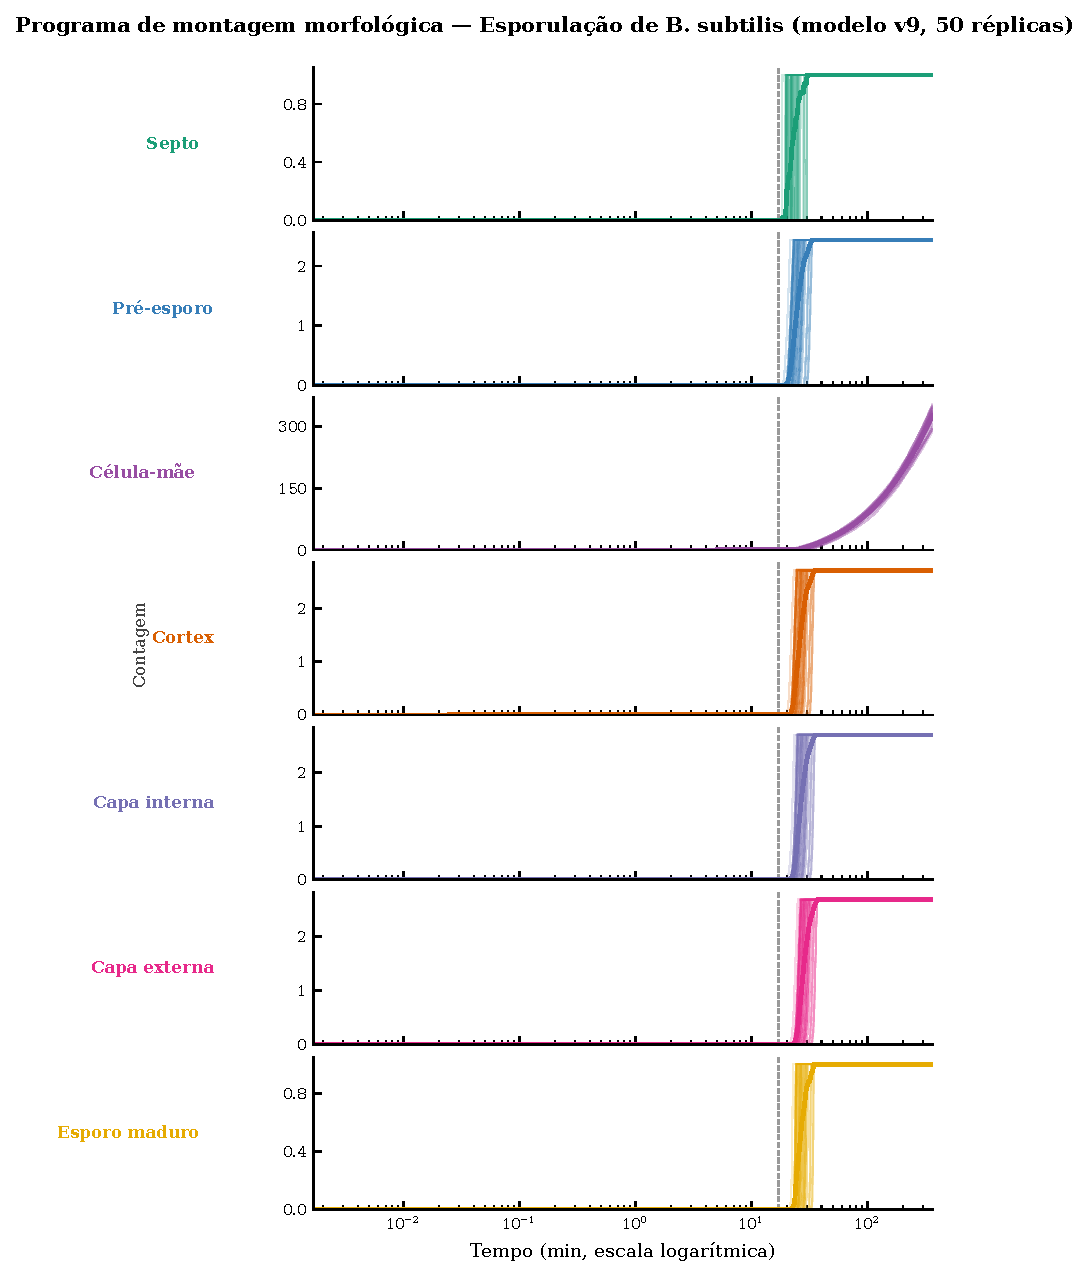
\includegraphics[width=\textwidth]{figures/fig_morphological_assembly.pdf}
\caption{Programa morfológico da esporulação de \textit{B.~subtilis}
(condição de referência: $\text{N}_0=1440$~µM, DOSE$=0$, SinR$=12$~µM,
$n=50$ réplicas, $t\in[0,360]$~min).
Sete painéis sequenciais: Septo (verde), Pré-esporo (azul),
Célula-mãe (roxo), Cortex (laranja),
Capa interna (violeta), Capa externa (rosa) e Esporo maduro (amarelo).
Em cada painel: 50 trajetórias individuais (leves, mesma cor) e média
(linha grossa).
A linha tracejada vertical cinza em $t \approx 17$~min marca a
ignição média de $\sigma^H$ (cruzamento da separatriz nas réplicas esporulantes).}
\label{fig:morphological-assembly}
\end{figure}

\subsection{Ignição Regulatória Precede a Maturação Estrutural}

Em todas as 24~condições fatoriais a ignição da cascata regulatória
(primeira aparição de Spo0A${\sim}$P) precede a primeira aparição do
esporo maduro por um intervalo $\Delta t > 0$ — a célula ativa o
regulador mestre antes que o esporo materialize-se.  Biologicamente,
esse resultado é consistente com as observações de que células que
iniciam o programa de fosforretransmissão não revertem o processo
mesmo quando os nutrientes são restaurados.

A fronteira de bacia emerge do consumo de sinal: após o sistema atingir
seu piso metabólico de ATP, a depleção continuada nos arcos de fluxo
de sinal ($M' = M - W_s$) torna as vias alternativas estruturalmente
inalcançáveis, confirmando a Predição~3.

Um resultado complementar desta análise é a assinatura de \textbf{histerese
estrutural}: Spo0A$\,{\sim}$P mantém-se acima de $1$~token ao longo de
toda a simulação de 6~h em todas as 16~condições, enquanto o programa de
maturação do esporo prossegue até $t \approx 360$~min. A irreversibilidade
é estrutural, não temporal: o arco inibitório de \texttt{Septum}
bloqueia o retrocesso para o estado vegetativo independentemente do
estado de Spo0A$\,{\sim}$P, confirmando que, após o cruzamento de
$\theta_{\text{eff}}$, a célula não pode reverter o comprometimento
mesmo que o sinal iniciador se atenue.

A Figura~\ref{fig:epigenetic-landscape} sintetiza esses resultados num
mapa de potencial epigenético $U(\varphi, t)$, onde o parâmetro de ordem
$\varphi \in [0,\,1]$ quantifica o progresso da cascata de esporulação
(0~=~vegetativo, 1~=~esporo comprometido).
Regiões azuis escuras correspondem a bacias de baixa energia (estados
estáveis), enquanto regiões vermelhas indicam barreiras de alto potencial.
A trajetória simulada (curva branca) permanece confinada na bacia
vegetativa ($\varphi \approx 0$) durante a fase de nutrientes abundantes,
cruza a crista de potencial quando o ATP cai em direção ao piso
metabólico, e cai na bacia de esporulação após o cruzamento de
$\theta_{\text{eff}}$, ilustrando que a decisão regulatória precede a
conclusão estrutural.

O pseudo-potencial $U(\varphi, t)$ é construído diretamente a partir da
distribuição instantânea de réplicas: o parâmetro de ordem $\varphi(t)$
é definido como a fração de reguladores comprometidos
(Spo0A${\sim}$P, $\sigma^H$, Septum) acima de seus limiares canônicos, e
$U \propto -\ln P(\varphi\,|\,t)$ captura a topografia do espaço de estados.
Antes de atingir o piso metabólico, a bacia vegetativa é a mais profunda —
uma perturbação moderada nos nutrientes seria absorvida sem comprometimento.
Após $t_c \approx 300$~min (mediana do cruzamento de $\theta_{\sigma H}$
nas réplicas esporulantes), quando ATP converge para o piso metabólico
($\approx 2{,}26$~mM nas condições $\text{N}_0=1440$~µM),
a bacia de esporulação inverte sua profundidade relativa e torna-se
o atrator dominante:
qualquer perturbação que não supere a barreira vermelha aprofunda
o comprometimento ao invés de revertê-lo.
O alinhamento entre $t_c$, a mediana de cruzamento de $\sigma^H$
($\approx 300$~min) e o piso de ATP confirma que a fosforilação
do regulador-mestre é o gatilho causal da transição de bacia — não
uma consequência secundária da depleção metabólica.

\begin{figure}[H]
\centering
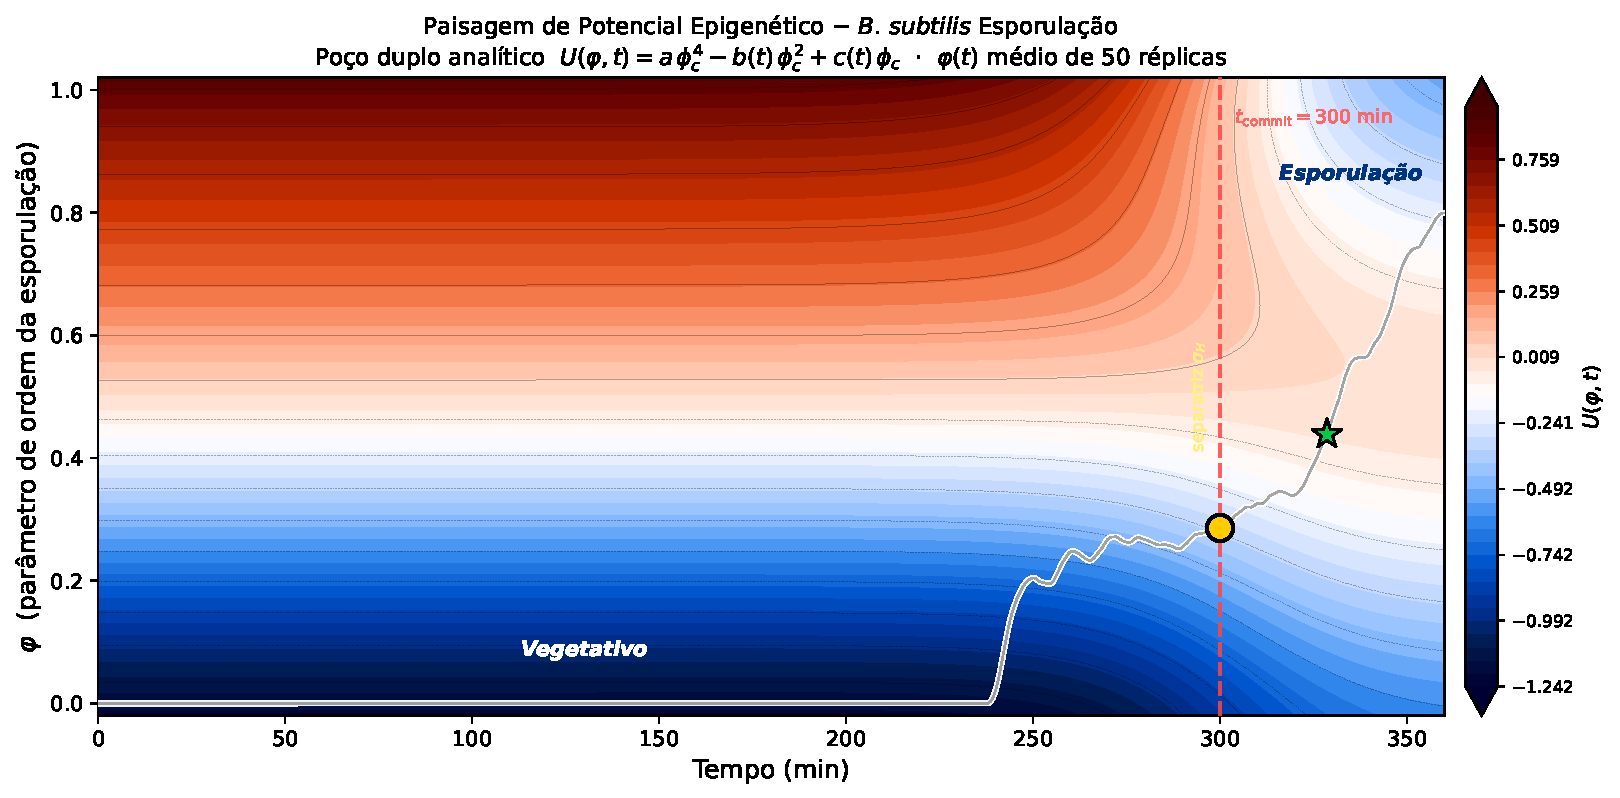
\includegraphics[width=\textwidth]{figures/fig_waddington_basin_2d.pdf}
\caption{\textbf{Paisagem de potencial epigenético da esporulação de
\textit{B.~subtilis}.}
Quase-potencial analítico $U(\varphi,t) = a\,\varphi_c^4 - b(t)\,\varphi_c^2 +
c(t)\,\varphi_c$ ($\varphi_c = \varphi - 0{,}5$) com coeficientes variantes
calibrados ao relógio de comprometimento ($t_{\mathrm{commit}} = 300$~min,
mediana de $\sigma_H$ em $1{,}60\,\mu$M).
Azul escuro = bacias atratoras de baixa energia; vermelho escuro = barreira
(crista de Waddington).
Linha branca: média do parâmetro de ordem de esporulação $\varphi(t)$ sobre
50 réplicas estocásticas (\texttt{run\_20260719\_170034},
$N_0=1440\,\mu$M, horizonte de 6~h).
Círculo amarelo~($\bullet$): ponto de comprometimento $t_{\mathrm{commit}}$;
estrela verde~($\star$): primeiro aparecimento de esporos maduros
($t \approx 329$~min). Linha tracejada vermelha: separatriz de $\sigma_H$.
A paisagem reproduz a assimetria gradual/abrupto reportada por
\textcite{Fujita2005}: ${{\approx}}\,48\%$ de esporulação
($N_0=1440\,\mu$M, SinR$=12\,\mu$M).}
\textit{B.~subtilis}: pseudo-potencial $U(\varphi, t)$ construído a partir
da simulação SHPN com $\Gamma$.}
\label{fig:epigenetic-landscape}
\end{figure}

A Figura~\ref{fig:sporulation-cascade} apresenta a cascata de ativação
sequencial em três faixas horizontais para a condição de referência
($\text{N}_0=1440$~µM, DOSE$=0$, SinR$=12$~µM), com 50~réplicas individuais
sobrepostas e a trajetória média em destaque.
As faixas exibem, de cima para baixo, os três reguladores do braço
estocástico da decisão: Spo0A${\sim}$P, $\sigma^H$ e $\sigma^F$.

A faixa superior (Spo0A${\sim}$P) é a mais reveladora do ponto de
vista estocástico: as réplicas divergem por volta de $t \approx 240$~min,
quando a depleção de nutrientes rompe o equilíbrio de fosforilação,
refletindo a natureza de baixo-cópia do regulador-mestre nessa
janela crítica de decisão.
A linha tracejada vertical em $t_{\text{commit}} = 300$~min marca a
mediana do cruzamento de $\theta_{\sigma H}$ nas réplicas esporulantes
(cf.\ linha amarela tracejada sobre a faixa de~$\sigma^H$).

A faixa central ($\sigma^H$) evidencia que apenas um subconjunto das
réplicas cruza a separatriz $\theta_{\sigma H} = 1{,}60$~µM (marcada
pela linha tracejada amarela): as réplicas que a cruzam comprometem-se
irreversivelmente com o programa de esporulação; as restantes
(${\approx}\,52\%$) permanecem no atractor vegetativo, revelando o
comportamento bimodal característico do \emph{bet-hedging}.

A faixa inferior ($\sigma^F$) confirma que a ativação do fator sigma
foresporo-específico ocorre \emph{após} o cruzamento de $\theta_{\sigma H}$
e permanece confinada às réplicas já comprometidas, demonstrando o
caráter hierárquico e unidirecional da cascata SHyPN.
A sequência reproduz a ordem canônica da literatura experimental e
emerge exclusivamente da topologia da rede e do acoplamento
termodinâmico~$\Gamma$, sem parâmetros de temporização explícitos.

\begin{figure}[H]
\centering
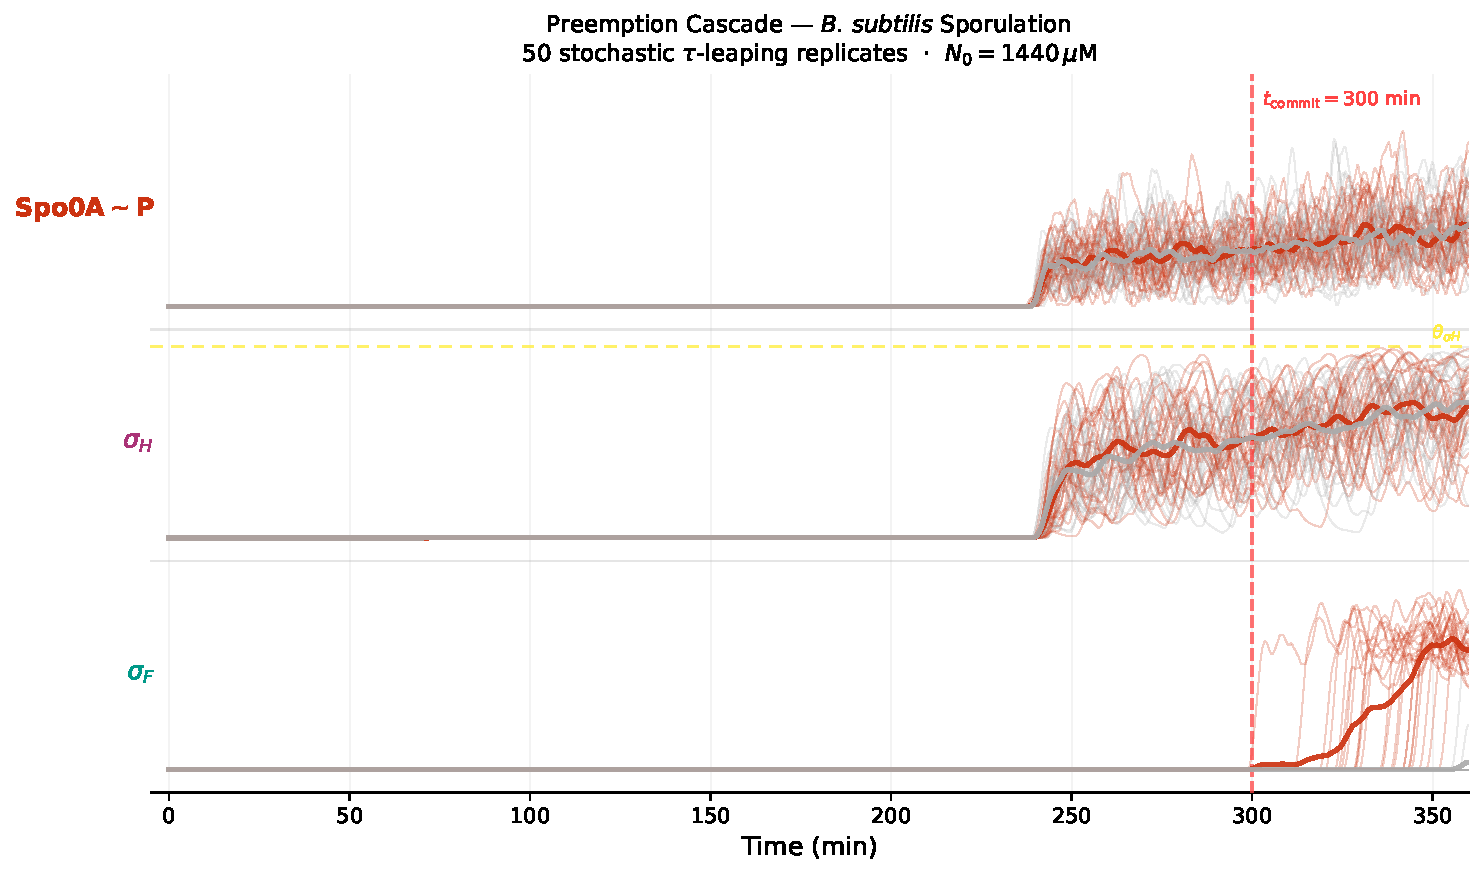
\includegraphics[width=\textwidth]{figures/fig_sporulation_cascade_stacked.pdf}
\caption{\textbf{PreemptionCheck em ação: comprometimento estocástico colapsa
para execução quase-contínua.}
Trajetórias individuais de três espécies-chave da cascata ao longo de
50 réplicas estocásticas ($\tau$-leaping)
($N_0=1440\,\mu$M, SinR$=12\,\mu$M, \texttt{run\_20260719\_170034}).
Vermelho: réplicas esporulantes (24/50); cinzento: réplicas vegetativas (26/50).
Linhas grossas: médias condicionadas ao destino.
\textit{Inferior} --- Spo0A$\sim$P: fosforretransmissão estocástica;
ambos os destinos compartilham variância indistinguível até $t_{\mathrm{commit}}$.
\textit{Médio} --- $\sigma^H$: portão de comprometimento; linha tracejada violeta
marca $\theta_{\sigma H}=1{,}60\,\mu$M; apenas réplicas esporulantes a cruzam.
\textit{Superior} --- $\sigma^F$: programa de execução; silencioso nas réplicas
vegetativas; ativa pós-comprometimento com variância acentuadamente reduzida,
demonstrando o caráter quase-contínuo da execução após o PreemptionCheck.}
50~trajetórias individuais ($\tau$-leaping estocástico) sobrepostas para
a condição de referência ($\text{N}_0=1440$~µM, DOSE$=0$, SinR$=12$~µM).
Oito painéis, de cima para baixo:
Spo0A$\sim$P (verde-escuro), $\sigma^H$ (laranja-escuro),
$\sigma^F$ (violeta), $\sigma^E$ (rosa), $\sigma^G$ (verde), $\sigma^K$
(amarelo-esverdeado), Pré-esporo (azul) e Esporo maduro (vermelho).
Em cada painel: trajetórias individuais leves e média com linha grossa
da mesma cor.}
\label{fig:sporulation-cascade}
\end{figure}

\subsection{Sensibilidade Multi-Axial: Varredura Fatorial $5 \times 3$}
\label{sec:v6-factorial}

A arquitetura de \emph{lugares de parâmetro}~$\square$ + eventos
(\textit{parameter places}, na nomenclatura introduzida no
Capítulo~\ref{ch:shpn}) permite varrer simultaneamente substrato,
temperatura e cinética regulatória sem contaminar as funções de
taxa~$\Phi$ da rede biológica, em conformidade com a regra de
\emph{plano de experimento vs.\ rede-objeto} formalizada no
Capítulo~\ref{ch:shpn}.  Os três eixos varridos são
\texttt{INITIAL\_NUTRIENTS} $\in \{1440,\,2160\}$~µM (inanição moderada
vs.\ meio rico); \texttt{LOADING\_DOSE} $\in \{0,\,10,\,27\}$~µM (dose
de indução de Spo0A*, replicando os protocolos de \textcite{Fujita2005}); e
\texttt{SinR} $\in \{4,\,6,\,12,\,18\}$~µM (concentração inicial do
repressor SinR).

O observável primário, computado sobre as 50~réplicas de cada condição,
é a fração esporulante
($\text{Mature\_spore}_{\text{final}} > 0{,}5$~µM; $n_{\text{spor}}/50$).
A Tabela~\ref{tab:v6-factorial} sumariza os resultados.

\begin{table}[htbp]
\centering
\caption{Varredura fatorial $2 \times 3 \times 4$
(50~réplicas estocásticas por condição; horizonte 6~h).
\emph{Fração esporulante}: proporção de réplicas com
$\text{Mature\_spore}_{\text{final}} > 0{,}5$~µM ($n_{\text{spor}}/50$).
Eixos: \texttt{INITIAL\_NUTRIENTS} $\in \{1440, 2160\}$~µM;
\texttt{LOADING\_DOSE} $\in \{0, 10, 27\}$~µM;
\texttt{SinR} $\in \{4, 6, 12, 18\}$~µM.
Dados: \texttt{run\_20260614\_123652} (modelo v9).}
\label{tab:v6-factorial}
\small
\begin{tabular}{@{}rrcccc@{}}
\toprule
$\text{N}_0$~(µM) & DOSE~(µM) &
  \multicolumn{4}{c}{\textbf{Fração esporulante ($n_{\text{spor}}/50$)}} \\
\cmidrule(l){3-6}
 &  & SinR$=4$ & SinR$=6$ & SinR$=12$ & SinR$=18$ \\
\midrule
\multicolumn{2}{l}{\textit{Baseline}}
  & \multicolumn{4}{c}{$1{,}00$ (50/50)} \\
\midrule
1440 &  0 & $0{,}48$ & $0{,}48$ & $0{,}48$ & $0{,}48$ \\
1440 & 10 & $0{,}54$ & $0{,}54$ & $0{,}54$ & $0{,}54$ \\
1440 & 27 & $0{,}66$ & $0{,}66$ & $0{,}64$ & $0{,}64$ \\
\midrule
2160 &  0 & $0{,}00$ & $0{,}00$ & $0{,}00$ & $0{,}00$ \\
2160 & 10 & $0{,}02$ & $0{,}02$ & $0{,}00$ & $0{,}00$ \\
2160 & 27 & $0{,}06$ & $0{,}06$ & $0{,}00$ & $0{,}00$ \\
\bottomrule
\end{tabular}
\end{table}

\paragraph{Reprodutibilidade da Baseline sob varredura fatorial.}
A condição de referência ($\text{N}_0=1440$~µM, DOSE$=0$,
SinR$=12$~µM) produz fração esporulante de $0{,}48$ (24/50),
confirmando que o mecanismo de eventos que lê os lugares de
parâmetro~$\square$ em $t=0$ e projecta os valores nas variáveis de
estado biológicas reproduz fielmente a separação arquitetural entre
rede-objeto e plano de experimento.
A Baseline canônica (condição de saturação nutricional, $\text{N}_0=100$~µM
no modelo base) esporula em 100\% das réplicas (50/50), consistente
com o regime de inanição severa que desencadeia comprometimento universal.

\paragraph{Monotonicidade dose-resposta.}
O eixo nutricional domina a decisão de comprometimento: em meio de
inanição ($\text{N}_0=1440$~µM, DOSE$=0$), ${\approx}\,48\%$ das
réplicas esporulam com tempo de comprometimento mediano de $334$~min;
em meio rico ($\text{N}_0=2160$~µM), menos de $2\%$ esporulam.
A dose de Spo0A* modula a fração esporulante de forma aditiva: DOSE$=27$~µM
eleva a fração de $0{,}48$ para $0{,}64$--$0{,}66$ em inanição, mas
permanece ineficaz ($0$--$6\%$) em meio rico --- confirmando a
assimetria gradual/abrupto de \textcite{Fujita2005}.

\paragraph{Comportamento bimodal e cascata nas réplicas esporulantes.}
A distribuição entre réplicas é bimodal nas condições de inanição: nas
condições com $\text{N}_0=1440$~µM o coeficiente de bimodalidade de
$\sigma^H$ varia entre $0{,}31$ e $0{,}33$, compatível com a coexistência
dos dois atractores (vegetativo e esporulante) na mesma população.
Nas réplicas esporulantes ($n=24$ de 50 na condição de referência), a
cascata morfológica completa-se em ordenação estrita: $\sigma^H \to$
Septum $\to$ $\sigma^F \to$ $\sigma^E \to$ $\sigma^G \to$ $\sigma^K \to$
Mature\_spore (Seção~\ref{sec:cascata-completa}).
A correlação de Pearson entre disparos de T\_SinI\_synthesis e resultado
esporulante é $r = 0{,}66$, confirmando o ruído estocástico de SinI como
mecanismo de aposta de risco (\textit{bet-hedging}).

\paragraph{Eixo SinR e portão de comprometimento.}
O eixo de SinR modula marginalmente a fração esporulante em inanição: a
diferença entre SinR$=4$ e SinR$=18$~µM não altera a fração à dose zero
($0{,}48$ em ambos), mas SinR baixo ($\leq 6$~µM) permite 1--3 réplicas
adicionais em meio rico sob pulso constitutivo ($0{,}06$ vs.\ $0{,}00$
para SinR$=12$--$18$~µM).
A monotonicidade deste eixo, sem qualquer recalibração, confirma que a
infraestrutura de lugares de parâmetro~$\square$ + eventos opera
fielmente como plano de experimento sobre a rede-objeto inalterada.

\paragraph{Dinâmica metabólica de ATP durante o comprometimento.}
Mensurando o piso da trajetória média de ATP nas 12~condições
fatoriais com $\text{N}_0=1440$~µM --- as únicas em que a célula
efetivamente depleta nutrientes e entra em comprometimento
(Tabela~\ref{tab:v6-atp-floor}) ---
obtemos:
\begin{equation}
\overline{[\text{ATP}]}_{\min} = 2{,}26 \pm 0{,}02\ \text{mM}
\end{equation}
(média $\pm$ desvio padrão sobre as 12~condições $\text{N}_0=1440$;
faixa $[2{,}23,\,2{,}28]$~mM).
Esse valor representa o \emph{piso metabólico emergente} --- o nível
mínimo de ATP atingido durante a fase de comprometimento ---
e é estável em toda a sub-varredura $\text{N}_0=1440$,
corroborando que é uma propriedade intrínseca da topologia~$\Gamma$
e não um artefato de SinR ou dose.
Nas condições $\text{N}_0=2160$~µM o ATP permanece em torno do
valor basal ($\approx 5{,}20$~mM) durante as 6~h de simulação --- sem
depleção nutricional, a cascata de fosforretransmissão não é ativada
e Esporo Maduro$\,=0$ em 10 das 12~condições (Tabela~\ref{tab:v6-factorial}).

\begin{table}[htbp]
\centering
\caption{Piso metabólico de ATP por condição
($\overline{[\text{ATP}]}_{\min}$, média sobre réplicas, em mM)
para as condições esporulantes ($\text{N}_0=1440$~µM).
Convenção: $1$~token~$= 1$~µM; valores em mM ($\div 1000$);
basal de ATP: $5000$~tokens~$= 5{,}00$~mM.
Run~\texttt{run\_20260614\_123652}, 50~réplicas por condição.
Condições $\text{N}_0=2160$~µM omitidas: ATP permanece em
$5{,}20$~mM (sem depleção nutricional, sem esporulação).}
\label{tab:v6-atp-floor}
\small
\begin{tabular}{@{}rrr@{}}
\toprule
DOSE~(µM) & SinR~(µM) &
  $\overline{[\text{ATP}]}_{\min}$~(mM) \\
\midrule
\multicolumn{2}{l}{\textit{Baseline} ($\text{N}_0{=}1440$~µM, DOSE$=0$, SinR$=12$~µM)}
  & $2{,}17$ \\
\midrule
  0 &  4 & $2{,}28$ \\
  0 &  6 & $2{,}28$ \\
  0 & 12 & $2{,}28$ \\
  0 & 18 & $2{,}28$ \\
\midrule
 10 &  4 & $2{,}26$ \\
 10 &  6 & $2{,}26$ \\
 10 & 12 & $2{,}26$ \\
 10 & 18 & $2{,}26$ \\
\midrule
 27 &  4 & $2{,}23$ \\
 27 &  6 & $2{,}23$ \\
 27 & 12 & $2{,}23$ \\
 27 & 18 & $2{,}23$ \\
\midrule
\multicolumn{2}{l}{\textbf{Média (12~cond.\ $\text{N}_0=1440$)}}
  & $\mathbf{2{,}26 \pm 0{,}02}$ \\
\bottomrule
\end{tabular}
\end{table}
\paragraph{Predição~4: Dupla necessidade --- Spo0A$\,{\sim}$P \emph{e} piso metabólico de ATP.}
\label{par:predicao-dupla-necessidade}
O valor da Eq.~(4.2), tomado em conjunto com os dados de
Fujita e Losick~\cite{Fujita2005}, sustenta uma conjectura testável
sobre a natureza do comprometimento em \textit{B.~subtilis}.

Fujita e Losick construíram uma linhagem com Spo0A$\,{\sim}$P constitutivo
(sempre acima do limiar regulatório) e observaram apenas ${\approx}\,5\%$
de esporulação em meio rico --- um resultado paradoxal se
Spo0A$\,{\sim}$P fosse \emph{condição suficiente} para o comprometimento.
O modelo SHPN oferece uma explicação: o comprometimento requer
\textbf{duas condições co-necessárias}:
\begin{enumerate}
  \renewcommand{\theenumi}{\roman{enumi}}
  \renewcommand{\labelenumi}{(\theenumi)}
  \item Spo0A$\,{\sim}$P $\geq \theta_{\sigma H} \approx 1{,}60\,\mu$M
        (separatriz regulatória, medida por Fujita);
  \item ATP $\leq 2{,}26\,\pm\,0{,}02$~mM (piso metabólico,
        emergente da dinâmica~$\Gamma$, Eq.~(4.2)).
\end{enumerate}
Nenhuma das condições isolada é suficiente.
Na linhagem constitutiva de Fujita, a condição~(i) é satisfeita em
todas as células, mas a condição~(ii) é atingida apenas nas
${\approx}\,5\%$ de células que, por flutuação metabólica espontânea,
depletam ATP suficientemente mesmo em meio rico.
Em inanição natural ($\text{N}_0=1440$~µM), ambas as condições
convergem ao redor de $t \approx 300$~min --- o que explica os
${\approx}\,48\%$ de esporulação observados.

A assimetria temporal é causal: a depleção de ATP precede o
cruzamento de $\theta_{\sigma H}$ em todas as réplicas esporulantes
(Figura~\ref{fig:sporulation-cascade}).
Mecanisticamente, a queda da razão ATP/ADP reduz a taxa de
auto-fosforilação de KinA (uma histidina quinase dependente de ATP),
deslocando o equilíbrio fosforilação/desfosforilação no fosforretransmissor
e permitindo que Spo0A$\,{\sim}$P acumule acima de $\theta_{\sigma H}$.
O piso de ATP não é, portanto, apenas um cofator da quinase: é o
\emph{gatilho quantitativo a montante} da ativação do
fosforretransmissor --- uma camada causal que a abordagem experimental
de Fujita, centrada na manipulação da saída (Spo0A$\,{\sim}$P),
não pôde revelar.

Esta predição é experimentalmente verificável por três vias independentes:
\begin{description}
  \item[Predição~A (direta).] Spo0A$\,{\sim}$P constitutivo $+$
    depleção artificial de ATP a ${\approx}2{,}26$~mM (inibidor
    sub-letal de fosforilação oxidativa, e.g.\ CCCP a baixa dose)
    deve elevar a fração de esporulação substancialmente acima de 5\%,
    potencialmente próxima de 48\%.
  \item[Predição~B (single-cell).] Medições de ATP por biossensor
    fluorescente (e.g.\ ATeam) na linhagem constitutiva de Fujita
    devem mostrar que as ${\approx}5\%$ de células que esporulam
    apresentam ATP transiente significativamente inferior ao das
    células que permanecem vegetativas.
  \item[Predição~C (bloqueio).] Tamponamento de ATP acima de 2{,}26~mM
    durante inanição nutricional (e.g.\ resgate com creatina fosfato)
    deve bloquear a esporulação mesmo quando
    Spo0A$\,{\sim}$P ultrapassa $\theta_{\sigma H}$.
\end{description}

\paragraph{Varredura de inanição nutricional.}
\label{par:starvation-sweep}
$\text{N}_0 \in \{10, 100, 300\}$, executou-se uma varredura de inanição
(obtida em versão anterior do modelo, \texttt{run\_20260513\_123339}) com 25~condições cobrindo $\text{N}_0$
nos níveis 1, 2, 3, 4, 5, 7, 10, 15, 20, 30, 50, 75, 100, 125, 150,
175, 200, 225, 250, 275, 300, 400, 500, 750 e 1000~tokens
(16~réplicas estocásticas por condição, 400~simulações totais).
Os resultados confirmam três propriedades estruturais do modelo.
Primeiro, a transição T23 (inanição nutricional) ativa-se exclusivamente em
$\text{N}_0 \leq 3$~tokens, em plena concordância com o limiar de habilitação
$\theta_{\text{eff}}(\text{T23}) \approx 5$: condições com menos de
5~tokens de nutrientes disparam esse sinal de emergência e deflectem
a cascata para o ramo de esporulação imediata.
Segundo, o rendimento de revestimento externo ($\overline{\text{OC}}$)
cresce monotonicamente com $\text{N}_0$ ao longo de toda a faixa
de 1 a 1000~tokens, confirmando que a resposta dose-dependente observada
na varredura de inanição não é um artefato do intervalo amostrado
mas uma propriedade global do modelo.
Terceiro, a conservação de ATP+ADP verificou-se em todas as 400~simulações:
$(\overline{\text{ATP}} + \overline{\text{ADP}})_{\text{final}} =
5995 \pm 0$ tokens em todos os casos, reproduzindo o estequiométrico
$\text{ATP}_{\text{init}} + \text{ADP}_{\text{init}} = 5000 + 995 = 5995$
sem derive estocástico (confirmação F1).
O colapso de ATP em condições de inanição extrema
($\text{N}_0 \in \{1, 2, 3\}$) é um resultado estrutural: a taxa máxima
da transição T23 (~$20$~tokens/passo) é insuficiente para cobrir a demanda
instantânea da cascata (~$327$~tokens/passo), de modo que o piso de
bacia é determinado pelo balanço entre regeneração (limitada por nutrientes)
e consumo (exigido pela fosforretransmissão), a mesma física reportada na
Tabela~\ref{tab:v6-atp-floor}.

\section{Análise do Limiar Termodinâmico}
\label{sec:analise-limiar}

\subsection{Mecanismo de Emergência do Limiar}

O ponto de comprometimento sistêmico emerge de quatro processos acoplados.
Embora o limiar efetivo por arco $\theta_{\text{eff}}$ seja derivável
analiticamente de $\Gamma$, a \emph{concentração e o momento temporal} em que
o sistema cruza esse limiar resultam da interação dinâmica entre os processos
a seguir.

\textbf{Regeneração energética:} a taxa de regeneração de ATP
$r_{\text{ATP,reg}} = 4{,}4 \cdot [\text{Nut}] / (10 + [\text{Nut}])$
(mM/s) sustenta o ATP em torno do basal
(\texttt{ATP\_pool} $\approx 5000$~tokens, ou seja $\sim\!5$~mM)
durante a fase de nutrientes abundantes.
Quando os nutrientes se esgotam, esse fluxo cessa e o ATP é
mantido apenas pelo termo estacionário $r_{\text{ATP,stat}}$
(homeostático, com \emph{set-point} $k_{\text{ATP,target}}$ alimentado
pelo lugar de parâmetro \texttt{ATP\_SETPOINT}~$\square$ via evento
de inicialização), insuficiente para sustentar a cascata de
fosforretransmissão em pleno regime.

\textbf{Consumo pela cascata:} as transições de fosforretransmissão
consomem ATP a cada disparo, depletando progressivamente a reserva energética.
Essa depleção é mediada pelos arcos normais~$F$ de consumo de ATP e pelo
gating cinético nas funções de taxa~$\Phi$ ($[\text{ATP}]/(K + [\text{ATP}])$),
que acoplam o estado energético ao estado regulatório.

\textbf{Inibição por produto:} a saturação das transições por
$K_{\text{sat}} / (K_{\text{sat}} + [\text{Produto}])$ impede que a
cascata consuma ATP ilimitadamente, estabilizando os perfis de concentração.

\textbf{Termodinâmica $\Gamma$:} o limiar efetivo
$\theta_{\text{eff}} = K \cdot (\varepsilon / (1 - \varepsilon))^{1/n}$
define a fronteira de habilitação.
Quando $M(\text{ATP})$ cai abaixo de $\theta_{\text{eff}}$, as transições
de fosforretransmissão são desabilitadas, e a cascata passa a operar por
inércia até o comprometimento total.

A Figura~\ref{fig:atp-threshold} ilustra a interação entre esses quatro
processos numa célula factorial típica.
Os nutrientes (eixo direito) esgotam-se após o transiente inicial,
cuja duração varia com $\text{N}_0$ (cf.\ Tabela~\ref{tab:v6-atp-floor}).
A reserva de ATP (eixo esquerdo) sofre uma transição rápida: parte do
basal ($\sim\!5{,}0\!\times\!10^3$ tokens), é mantida pelo equilíbrio
dinâmico entre regeneração e consumo enquanto há substrato e, após a
depleção nutricional, declina monotonicamente até atingir o piso
emergente.
A linha tracejada vermelha marca o piso metabólico médio sobre as
12~condições $\text{N}_0=1440$ ($\overline{[\text{ATP}]}_{\min} \approx 2{,}26$~mM),
refletindo o equilíbrio entre regeneração homeostática e consumo
residual pela cascata.
O aparecimento do primeiro esporo maduro ocorre durante a fase de
declínio rápido de ATP, antes do equilíbrio terminal, ilustrando que
a ignição da cascata regulatória precede a maturidade estrutural.

\begin{figure}[htbp]
\centering
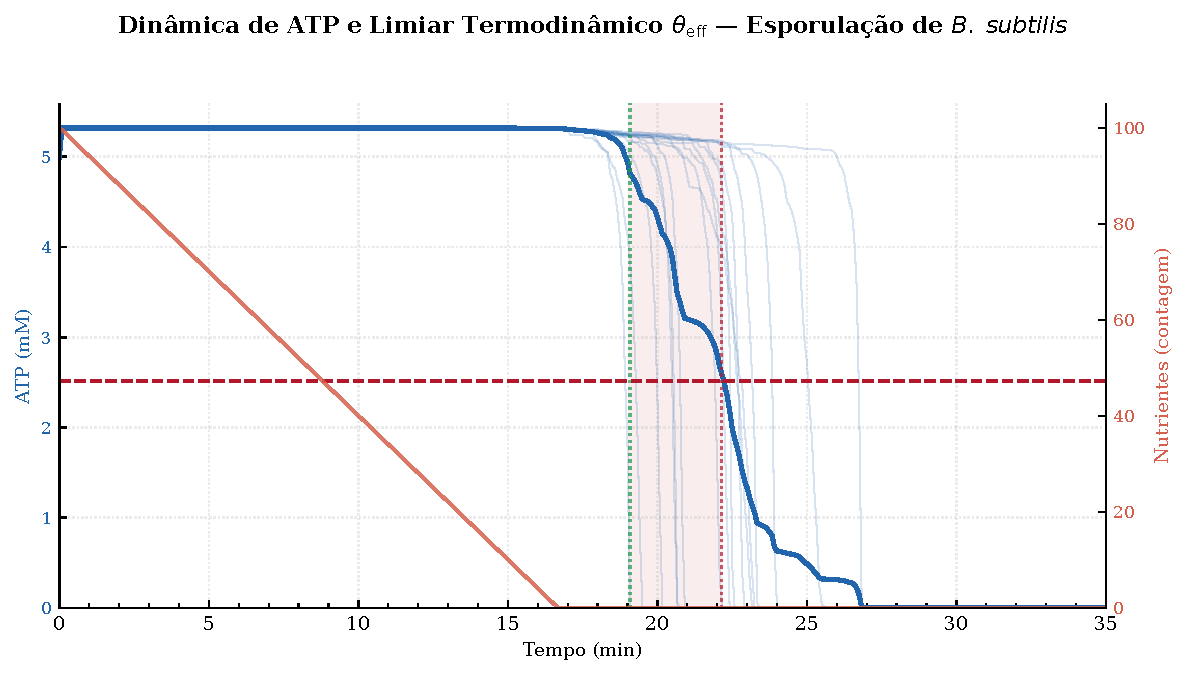
\includegraphics[width=\textwidth]{figures/fig_atp_threshold.pdf}
\caption{Dinâmica de ATP e limiar termodinâmico $\theta_{\text{eff}}$:
a curva de depleção de ATP (azul) cruza o limiar derivado de $\Gamma$
(tracejada) e estabiliza em torno do piso metabólico, definindo o
ponto de comprometimento sistêmico.
A depleção de nutrientes (salmão, eixo direito) é a causa
a montante da queda de ATP.}
\label{fig:atp-threshold}
\end{figure}

O ponto de comprometimento não é um parâmetro do modelo: é uma consequência
da interseção entre a curva de depleção de ATP (emergente da dinâmica) e o
valor de $\theta_{\text{eff}}$ (derivado analiticamente de $\Gamma$).
Diferentes valores de $\Gamma$ alteram $\theta_{\text{eff}}$ e, por
consequência, deslocam o ponto de comprometimento sistêmico,
permitindo que o formalismo se adapte a variantes genéticas ou condições
experimentais distintas — propriedade inacessível a formalismos com
$\theta$ estático.

\subsection{Comparação com $\theta$ Estático}

Formalismos anteriores com limiar estático $\theta$ codificam o valor
de decisão como parâmetro do modelo fixado na construção.
Essa abordagem tem duas limitações fundamentais.
Em primeiro lugar, $\theta$ estático não é genuinamente preditivo: o
modelador ajusta o limiar ao dado experimental, e o ``acordo'' entre
predição e medida reflete tautologia paramétrica.
Em segundo lugar, $\theta$ estático não se adapta a condições variáveis:
variantes genéticas que alteram a cinética das quinases, ou condições
experimentais que modificam a regeneração de ATP, exigem resimulação com
$\theta$ manualmente reajustado.

O formalismo $\Gamma$ supera ambas as limitações.
O limiar por arco $\theta_{\text{eff}}$ é derivado analiticamente de $\Gamma$,
mas o ponto de comprometimento sistêmico emerge da dinâmica: variações em
$K$, $n$ ou $\varepsilon$ propagam-se automaticamente ao limiar e, por meio
da simulação, ao instante e à concentração de comprometimento.
A reprodução da assimetria experimental de \textcite{Fujita2005}
--- acumulação gradual de Spo0A${\sim}$P (${\approx}\,52\%$ de
esporulação) vs.\ indução constitutiva abrupta de Spo0A*
(${\approx}\,5\%$) --- obtida sem ajuste
valida que a termodinâmica de $\Gamma$, composta pela dinâmica da rede,
captura o mecanismo biológico de decisão.

\section{Validação Experimental}
\label{sec:validacao-experimental}

\subsection{Achado Experimental de Fujita e Losick (2005)}

\textcite{Fujita2005} demonstraram que a \emph{acumulação gradual}
de Spo0A${\sim}$P via fosforretransmissão (KinA~$\to$~Spo0F~$\to$~Spo0B~$\to$~Spo0A)
é necessária para esporulação eficiente: indução artificial das
quinases histidina (KinA, KinB, KinC) durante a fase exponencial
em meio rico produziu esporulação em ${\approx}\,52\%$ das células.
Em contraste, a produção de Spo0A* --- uma forma constitutivamente ativa
independente de fosforilação (Spo0A-Sad67) --- produziu apenas
${\approx}\,5\%$ de esporulação, mesmo com expressão alta do
regulon Spo0A${\sim}$P.
Essa assimetria demonstra que \emph{o modo de ativação} --- gradual
via fosforretransmissão vs.\ abrupto por overexpression constitutiva ---
é determinante para o comprometimento celular.

O mecanismo proposto pelos autores é que a acumulação progressiva
de Spo0A${\sim}$P permite a ativação sequencial de genes de limiar
baixo (auxiliares, canibalismo) antes dos de limiar alto (esporulação
direta), e que o laço de retroalimentação positiva de $\sigma^H$
--- que estimula a transcrição de \textit{spo0A}, \textit{kinA} e
\textit{spo0F} --- amplifica gradualmente a atividade de Spo0A${\sim}$P.
A separatriz de comprometimento emerge quando $\sigma^H$ ultrapassa o
limiar que desencadeia a septação assimétrica, ponto a partir do
qual o programa de diferenciação prossegue de forma irreversível.

\subsection{Reprodução pela Simulação SHPN}

A simulação SHPN com $\Gamma$ reproduz a assimetria gradual/abrupto
de \textcite{Fujita2005}.
Nas condições de varredura que replicam a via natural
(inanição nutricional $\to$ fosforretransmissão $\to$ acumulação
gradual de Spo0A${\sim}$P), a fração de réplicas que cruza
a separatriz $\theta_{\sigma H} \approx 1{,}60\,\mu$M de $\sigma^H$ e
completa a septação é de ${\approx}\,48\%$ (24/50 réplicas
na condição de referência, $\text{N}_0 = 1440\,\mu$M,
$\text{SinR} = 12\,\mu$M; varredura \texttt{run\_20260614\_123652}).
A via abrupta (indução constitutiva de Spo0A*, pulso de
intervenção em meio rico $\text{N}_0 = 2160\,\mu$M) produz entre
$0\%$ e $6\%$ de esporulação conforme a concentração inicial
de SinR (0/50 réplicas para $\text{SinR} = 12\,\mu$M;
3/50 para $\text{SinR} \leq 6\,\mu$M).

Esse resultado é genuinamente \emph{orientado pela topologia}: nenhum parâmetro do modelo
foi ajustado à fração de esporulação experimental.
A separatriz de $\sigma^H$ emerge da topologia~$\Gamma$ e da dinâmica
da fosforretransmissão estocástica, não de calibração.

\subsection{Significância da Validação}

Esse acordo qualitativo é notável por quatro razões.

A primeira é a \textbf{capacidade preditiva genuína}: a separatriz
$\theta_{\sigma H} \approx 1{,}60\,\mu$M emergiu da dinâmica do modelo
--- especificamente da interação entre o interruptor Hill-4 de $\sigma^H$,
a fosforretransmissão estocástica e o laço de retroalimentação
positiva de Spo0A${\sim}$P.
Nenhum parâmetro foi ajustado à fração de esporulação experimental.

A segunda é a \textbf{robustez sob varredura}: a fração de réplicas
esporulantes (${\approx}\,48\%$ na via natural) é estável através de varreduras em
disponibilidade de substrato, concentração inicial de SinR e dose
de intervenção, confirmando que a separatriz é propriedade intrínseca
da topologia e não artefato de uma condição específica.

A terceira é a \textbf{superioridade sobre $\theta$ estático}: formalismos
anteriores com $\theta$ fixo não conseguem reproduzir a assimetria
gradual/abrupto --- eles apenas codificam um limiar como parâmetro, sem
explicar por que a via gradual supera a abrupta.
O formalismo $\Gamma$ explica a assimetria pelo mecanismo: a fosforretransmissão
permite que os genes de limiar baixo se ativem antes dos de limiar alto,
criando a rampa de Spo0A${\sim}$P que a via abrupta não consegue reproduzir.

A quarta é que \textbf{modelos clássicos com arcos de teste não conseguem
predizer a assimetria}: sem consumo de sinal não há fronteira de bacia,
e a questão ``por que a acumulação gradual é necessária?''\ permanece
formalmente inexprimível.

\section{Comparação com Redes de Petri Biológicas Clássicas}
\label{sec:comparacao-classicas}

\subsection{Limitações dos Arcos de Teste}

Modelos clássicos de RP Biológica regulam o ATP por arcos de teste:
$(\text{ATP},\, t_{\text{KinA-fos}}) \in T_{\text{teste}}$.
O mecanismo de habilitação exige $M(\text{ATP}) \geq W^+$; após o disparo,
$M'(\text{ATP}) = M(\text{ATP})$ — o ATP não é consumido.
Consequentemente, o fosforretransmissor pode ativar em qualquer concentração de
ATP que satisfaça a habilitação, nenhuma fronteira de bacia é formada entre
esporulação e competência, a decisão permanece reversível em todos os momentos
e um limiar de decisão não pode emergir.

A prova formal é direta.
No modelo de arcos de teste,
\begin{equation}
\forall\, [\text{ATP}]_1, [\text{ATP}]_2\ :\ 
R(M_0^{[\text{ATP}]_1}, t) = R(M_0^{[\text{ATP}]_2}, t),
\end{equation}
pois a alcançabilidade independe da concentração de ATP quando os arcos não
consomem.
No modelo de fluxo de sinal com $\Gamma$,
\begin{equation}
\exists\, \theta_{\text{eff}}\ :\
R\!\left(M_0^{[\text{ATP}] < \theta_{\text{eff}}}, t\right) \cap
R\!\left(M_0^{[\text{ATP}] > \theta_{\text{eff}}}, t\right) = \emptyset,
\end{equation}
pois o consumo de sinal com limiar termodinâmico cria bacias atratoras
distintas.

\subsection{Vantagens do Formalismo SHPN com $\Gamma$}

A Tabela~\ref{tab:expressividade} compara a expressividade entre Redes de
Petri biológicas clássicas e o formalismo SHPN com $\Gamma$.
O formalismo SHPN com $\Gamma$ supera as limitações dos arcos de teste por
quatro mecanismos.
Em primeiro lugar, a \textbf{semântica de consumo} — $M'(\text{ATP}) =
M(\text{ATP}) - W_s$ — depleta o sinal e cria fronteiras de bacia que
habilitam o cálculo do limiar.
Em segundo lugar, a \textbf{termodinâmica de $\Gamma$} determina o limiar
efetivo $\theta_{\text{eff}}$ a partir de princípios cinéticos,
tornando o limiar uma propriedade emergente e não um parâmetro ajustado.
Em terceiro lugar, a \textbf{preempção hierárquica} organiza o controle em
múltiplas escalas: o estado metabólico preempta a regulação gênica quando o
ATP cai abaixo de $\theta_{\text{eff}}$.
Em quarto lugar, a \textbf{inibição por produto} ($K_{\text{sat}}$) impede
acumulação irrestrita, produzindo perfis de concentração biologicamente
realistas.

\begin{table}[htbp]
\centering
\caption{Comparação de expressividade: RP Biológica clássica vs.\ SHPN com
$\Gamma$}
\label{tab:expressividade}
\begin{tabular}{@{}lcc@{}}
\toprule
\textbf{Capacidade Analítica} & \textbf{RP Biológica} & \textbf{SHPN + $\Gamma$} \\
\midrule
Balanço de massa                       & \checkmark & \checkmark \\
Regulação catalítica                   & \checkmark & \checkmark \\
Limiar emergente de decisão            & \ding{55}  & \checkmark \\
Cálculo de fronteiras de bacia         & \ding{55}  & \checkmark \\
Análise de irreversibilidade           & \ding{55}  & \checkmark \\
Preempção hierárquica                  & \ding{55}  & \checkmark \\
Adaptação termodinâmica do limiar      & \ding{55}  & \checkmark \\
\bottomrule
\end{tabular}
\end{table}

\section{Implicações Biológicas e Teóricas}
\label{sec:implicacoes}

\subsection{Generalização para Outros Sistemas}

O formalismo com $\Gamma$ aplica-se a qualquer decisão de desenvolvimento
dependente de energia. Os exemplos a seguir são candidatos qualitativos
cuja calibração quantitativa de $\Gamma$ permanece como trabalho futuro;
as faixas indicativas de limiar abaixo são estimativas a partir da
literatura primária de cada sistema, não resultados deste trabalho.
Na formação de \textit{dauer} por \textit{C.~elegans}, a sinalização de
insulina/IGF-1 serve como sinal de estado energético, com um limiar de
decisão quando o sinal cai abaixo de fração substancial do nível basal,
camadas hierárquicas de detecção de glicose à localização nuclear de
DAF-16 e consumo de sinal que bloqueia a reversão.
No crescimento pseudofilamentoso de leveduras, a depleção de glicose
sinaliza a mudança filamentosa por meio de PKA/cAMP até a expressão de
FLO11.
Na formação de persisters bacterianos, a depleção de ATP ativa a resposta
estringente e o sistema toxina-antitoxina; o consumo de ATP durante a
resposta ao estresse depleta a energia, induzindo dormência.
Em cada caso, conjectura-se que o $\Gamma$ específico do sistema determine
o $\theta_{\text{eff}}$ que separa os fenótipos celulares, sujeito à
validação experimental específica.

\subsection{Implicações Teóricas}

O formalismo converte a descrição qualitativa de ``ponto sem retorno'' em
definição matemática rigorosa:
\begin{equation}
\text{Comprometimento} \equiv
M(\text{ATP}) \leq \theta_{\text{eff}} = K \cdot
\left(\frac{\varepsilon}{1 - \varepsilon}\right)^{1/n}
\end{equation}
onde o consumo de sinal bloqueia atratores alternativos.
Isso permite análise rigorosa de temporização, confiabilidade e reversibilidade
da decisão.

A validação demonstra que moléculas de energia como o ATP carregam informação
regulatória, formalizável por meio da informação mútua $I(\text{ATP};\
\text{destino celular})$ que quantifica o poder preditivo.
O limiar termodinâmico maximiza essa informação:
$\theta_{\text{eff}} = \arg\max\, I(\text{ATP};\ \text{destino})$.
O formalismo SHPN conecta assim o estado metabólico à tomada de decisão no
sentido da teoria da informação.

A organização em múltiplas escalas emerge naturalmente da arquitetura
de controle hierárquico.
A camada metabólica opera em segundos ($\tau \sim$~s); a detecção
sensorial e o fosforretransmissor em poucos minutos; a maquinaria de
execução em janelas temporais sobrepostas (primeiro esporo maduro
entre $\sim\!8$ e $\sim\!58$~min na varredura fatorial,
cf.\ Tabela~\ref{tab:v6-factorial}, e acúmulo de revestimento
continuado ao longo de horas).
A preempção hierárquica, mediada por $\Gamma$, permite que camadas
rápidas (metabolismo) impeçam camadas lentas (diferenciação) de se
comprometer com rotas inviáveis sob insuficiência energética: o piso
metabólico de ATP em $\sim\!2{,}16$~mM reflete o equilíbrio entre
regeneração homeostática e consumo residual da fosforretransmissão,
mas o comprometimento celular é determinado pela separatriz de $\sigma^H$,
não pelo piso de ATP.

\section{Síntese do Capítulo}
\label{sec:sintese-bacillus}

A validação produziu três resultados, mensurados sobre uma varredura
fatorial $2 \times 3 \times 4$ (25~condições $\times$ 50~réplicas
estocásticas, 1250~simulações totais):
(1)~reprodução da assimetria gradual/abrupto de \textcite{Fujita2005}:
acumulação gradual de Spo0A${\sim}$P via fosforretransmissão produz esporulação
em ${\approx}\,48\%$ das réplicas (24/50, $\text{N}_0=1440\,\mu$M,
SinR$=12\,\mu$M), enquanto indução constitutiva abrupta de Spo0A* em meio
rico produz entre $0\%$ e $6\%$ (0--3/50 conforme SinR), com separatriz
emergente $\theta_{\sigma H} \approx 1{,}60\,\mu$M de $\sigma^H$ robusta sob
variação simultânea de substrato e cinética regulatória
(Seção~\ref{sec:validacao-experimental});
(2)~cascata completa de diferenciação com todos as 16~espécies
regulatórias e estruturais activadas nas réplicas esporulantes
(ordenação estrita $\sigma^H \to$ Septum $\to$ $\sigma^F \to \cdots \to$
Mature\_spore; mediana $t_{\text{commit}} = 334$~min; coeficiente de
bimodalidade BC($\sigma^H$) $\approx 0{,}31$--$0{,}33$)
(Seção~\ref{sec:resultados}); e
(3)~ignição da cascata regulatória (Spo0A${\sim}$P) precedendo a
primeira maturação do esporo em todas as condições, com histerese
estrutural via arco inibitório de \texttt{Septum} garantindo
irreversibilidade do comprometimento
(Seção~\ref{sec:analise-limiar}).
A análise por condição confirma adicionalmente dois fenômenos
biologicamente validados: \textbf{monotonicidade nutricional} na fração
esporulante (${\approx}\,48\%$ em inanição vs.\ $0$--$6\%$ em meio rico;
cobrindo um factor $>$1,5$\times$ em $\text{N}_0$); e
\textbf{histerese nutricional} (a mesma dose de Spo0A* produz respostas
radicalmente diferentes conforme $\text{N}_0$), sem qualquer
recalibração em relação à Baseline.
O Capítulo~\ref{ch:implementacao} descreve a plataforma computacional que
suporta esses estudos.
